\section{Génomique à l'ère du Big Data}
\label{sec:db}
Avec l'évolution des méthodes de séquençage et la diminution des coûts, de plus en plus de projets de recherche s'appuient sur le séquençage des génomes pour faire des analyses de génomique comparée. Les chercheurs peuvent ensuite rendre ces séquences publiques et les déposer dans des banques de données (BD) de génomes, comme GenBank \cite{burks_genbank_1985}. GenBank est la BD de séquence du \textit{National Center for Biotechnology Information} (NCBI), toutes les séquences qui y sont soumises passent un contrôle d'intégrité et de qualité, avant d'être annotées automatiquement. Entre 2010 et 2025, le nombre de génomes stockés dans GenBank a connu une croissance exponentielle,  passant de quelques milliers à plus de 2,5 millions de génomes. (\autoref{fig:cumm_genbank}).

\begin{figure}[htbp]
    \centering
    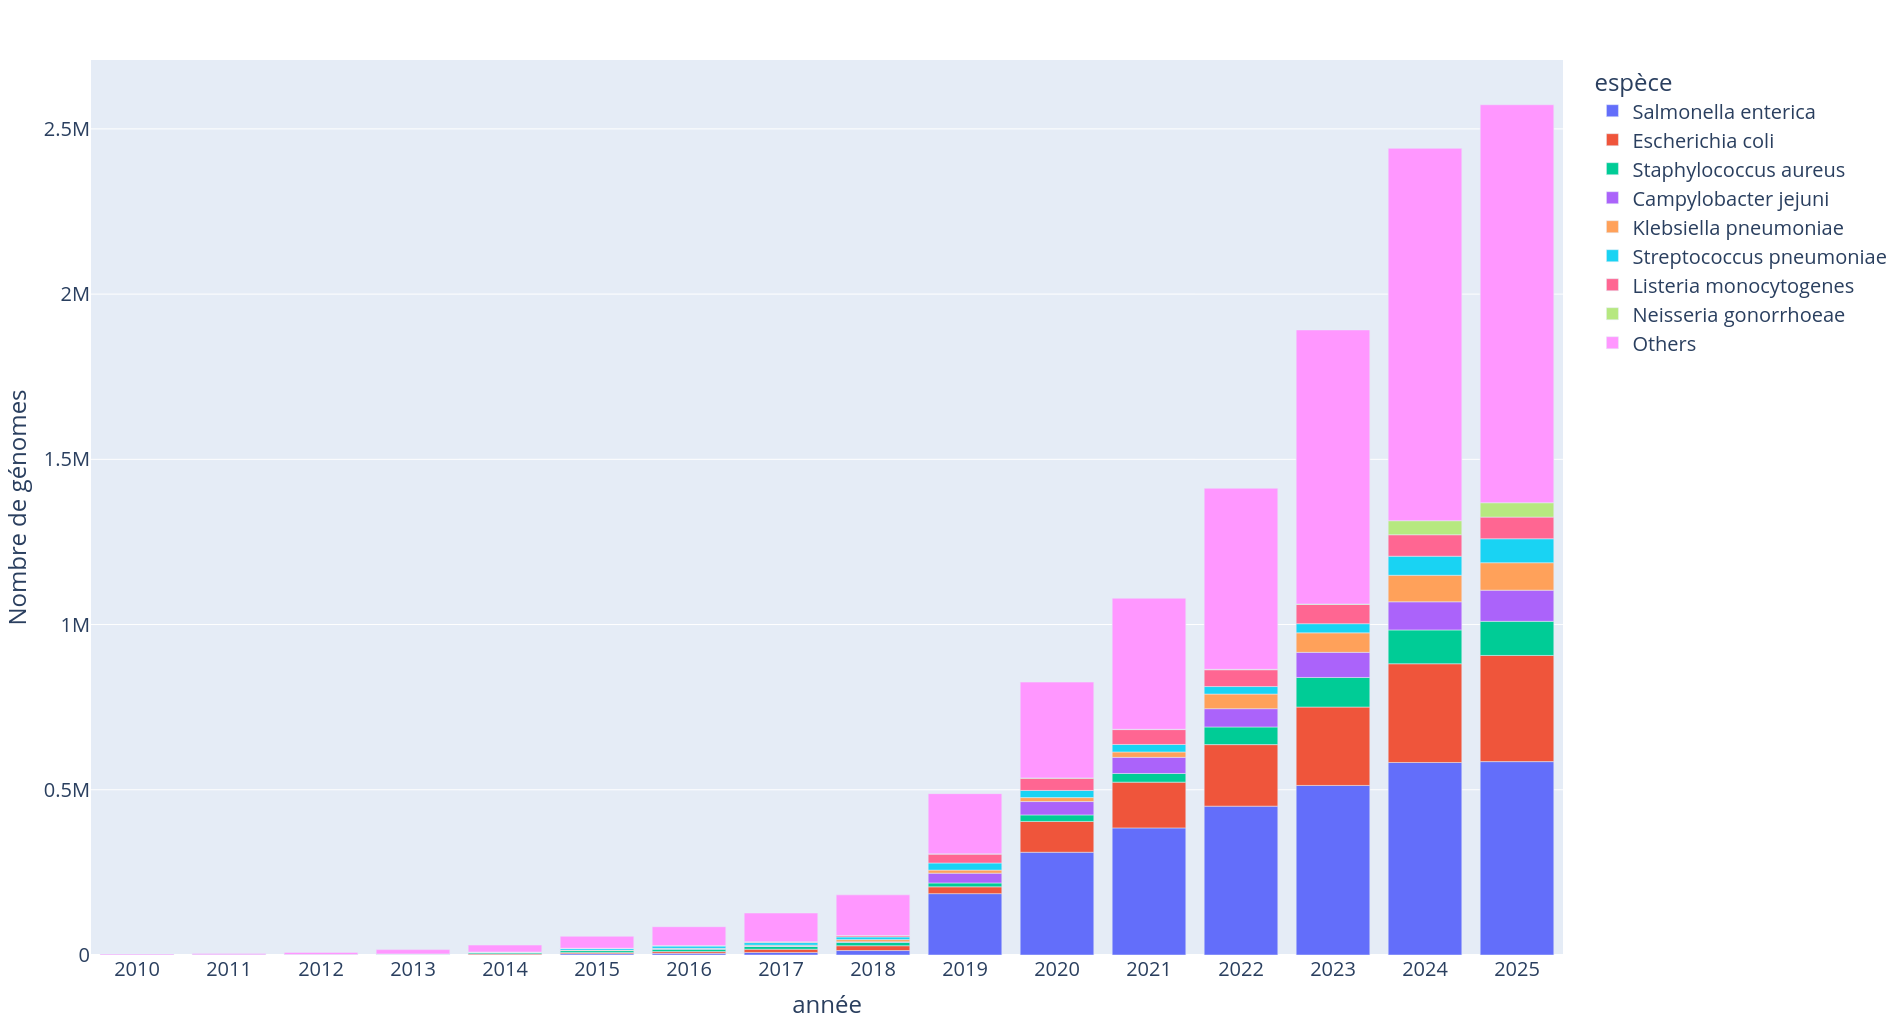
\includegraphics[width=\linewidth]{images/cummulativeGenomesGenBank.png}
    \caption[Nombre de génomes cumulés par an dans GenBank]{\textbf{Nombre de génomes cumulés par an dans GenBank.} Les génomes pris en compte sont uniquement ceux des procaryotes. Les espèces indiquées en légende sont les plus représentées dans GenBank. Construit avec l'outil drawbank \url{https://github.com/axbazin/drawbank}}
    \label{fig:cumm_genbank}
\end{figure}

À partir des génomes annotés, il est possible d'obtenir la traduction des gènes en séquences protéiques, prédire leurs fonctions, leurs structures\dots Toutes ces informations vont également être contenues dans des BD spécifiques pour aider aux analyses. Les BD peuvent aussi être thématiques, en contenant uniquement les génomes d'une espèce ou d'une région géographique, par exemple.

Avec l’essor du Big Data, les méthodes de génomique comparée vont être améliorées et adaptées afin d'analyser efficacement ce nouvel immense volume de données.
%La génomique doit alors s'adapter et profiter de ce vaste ensemble de données qu'est le \textit{Big Data}.

\subsection{Base de données génomiques}

L’existence et l’accessibilité des bases de données biologiques sont fondamentales pour l’annotation, la classification et l’analyse des séquences génomiques et protéiques. Parmi ces ressources, plusieurs se distinguent par leur spécialisation.

Parmi les bases de données de référence de génomes, RefSeq \cite{pruitt_ncbi_2007}, développée et maintenue par le NCBI, se distingue par la qualité et la fiabilité de ses annotations. Contrairement à GenBank, alimentée par des soumissions d’utilisateurs, RefSeq compile des séquences rigoureusement validées, incluant des ARN et des protéines issus d’une grande diversité d’organismes. Son processus de standardisation strict en fait une ressource incontournable pour la génomique comparative et une base essentielle pour des outils phares du NCBI, comme BLAST. En complément des séquences individuelles, RefSeq propose des ensembles complets de génomes annotés, notamment pour des organismes modèles et des pathogènes.

Dans le domaine des protéines, \textbf{UniProt} \cite{the_uniprot_consortium_uniprot_2025} est une ressource incontournable pour l’annotation et l’analyse des séquences protéiques. Elle est développée et maintenue par un consortium composé de l'\textit{European Bioinformatics Institute }(EMBL-EBI), le \textit{Swiss Institute of Bioinformatics} (SIB) et la \textit{Protein Information Resource} (PIR). Elle se divise en 3sections : (\textit{i}) \textbf{UniProtKB} (\textit{KnowledgeBase}), qui comprend des annotations détaillées sur les protéines et est divisé en \textbf{Swiss-Prot} (annotations manuelles et validées) et \textbf{TrEMBL} (annotations automatiques) \cite{apweiler_uniprot_2004,bairoch_swiss-prot_2004} ; (\textit{ii}) \textbf{UniRef} (\textit{UniProt Reference Clusters}), qui regroupe des séquences non redondantes à différents seuils de similarité \cite{suzek_uniref_2007}; (\textit{iii}) \textbf{UniParc} (\textit{UniProt Archive}), une archive complète de toutes les séquences protéiques connues, indépendamment de leur source. Cette base de données est essentielle pour la modélisation structurale des protéines, la découverte de cibles thérapeutiques et la génomique fonctionnelle.

\textbf{GTDB} (Genome Taxonomy Database) \cite{parks_standardized_2018} propose une taxonomie révisée des génomes procaryotes, fondée sur des analyses phylogénomiques. Contrairement aux approches classiques reposant sur des critères phénotypiques, GTDB utilise une approche purement génomique basée sur l'analyse comparée de 120 gènes marqueurs afin d’harmoniser la classification. Comme l’illustre la \autoref{fig:GTDB_tax}, cette approche permet d’obtenir une taxonomie plus homogène que celle du NCBI. De plus, GTDB intègre les génomes environnementaux et non cultivables issus de métagénomes, facilitant ainsi l’identification de nouvelles espèces et l’exploration de la diversité microbienne selon des critères plus objectifs.

\begin{figure}
    \centering
    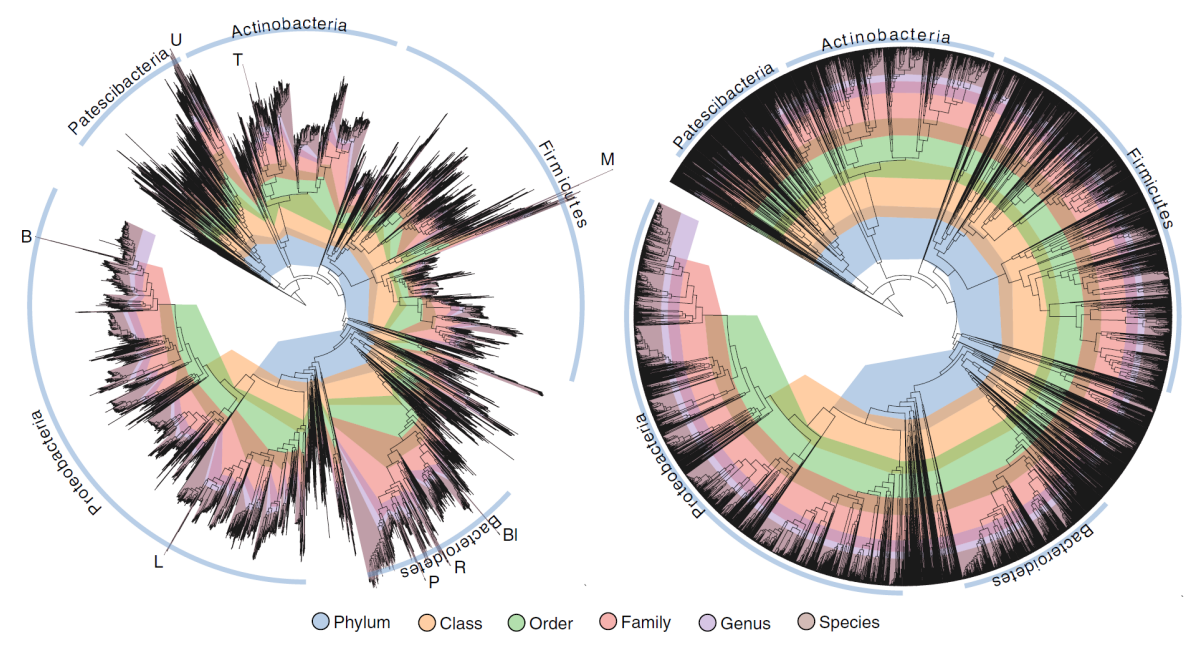
\includegraphics[width=.75\linewidth]{images/GTDB_taxonomie.png}
    \caption[Comparaison de l'homogénéité des rangs taxonomiques entre le NCBI et GTDB]{\textbf{Comparaison de l'homogénéité des rangs taxonomiques entre le NCBI et GTDB.} Les 2 figures représentent le même arbre avec à gauche la taxonomie proposée par le NCBI et à droite celle proposée par GTDB. Copié de \cite{gautreau_conceptualisation_2020} et adapté de \cite{parks_standardized_2018}}
    \label{fig:GTDB_tax}
\end{figure}

L’analyse des communautés microbiennes complexes repose sur des bases de données spécialisées comme \textbf{MGnify}\footnote{anciennement nommé EBI Metagenomics \cite{hunter_ebi_2014}} \cite{richardson_mgnify_2023}, une plateforme développée par l’EMBL-EBI dédiée à l’étude des données métagénomiques. Contrairement aux bases centrées sur des séquences génétiques isolées, MGnify s’intéresse aux microbiomes présents dans divers environnements tels que le sol, les océans, les eaux douces, le microbiote humain ou encore les milieux extrêmes. En plus de stocker des données, elle propose des outils bioinformatiques avancés pour l’assemblage, l’annotation et l’analyse fonctionnelle des communautés microbiennes. MGnify permet ainsi d’identifier les espèces présentes dans un échantillon via des approches de taxonomie basées sur l’ARNr 16S/18S, de prédire les fonctions métaboliques des microbiomes et d’étudier leurs interactions avec l’environnement. Cette ressource est devenue incontournable en écologie microbienne et en biotechnologie.

Dans le domaine de la résistance aux antibiotiques, CARD (\textit{Comprehensive Antibiotic Resistance Database}) \cite{mcarthur_comprehensive_2013} est une base de données spécialisée qui regroupe des informations sur les gènes de résistance, les mutations associées et les mécanismes moléculaires impliqués. Elle est notamment utilisée pour identifier les gènes de résistance dans des échantillons génomiques en utilisant l'outil RGI \cite{alcock_card_2023}, et métagénomiques grâce à l’outil CARPDM \cite{hackenberger_carpdm_2024}. CARD adopte une nomenclature standardisée basée sur l’ontologie ARO (\textit{Antibiotic Resistance Ontology}) pour classifier les résistances selon leur mode d’action et leur mode de transmission, facilitant ainsi l’étude et la surveillance des résistances aux antibiotiques.

Enfin, pour les chercheurs spécialisés dans l'étude des bactéries du genre Pseudomonas, la \textbf{Pseudomonas Genome Database} (PGD) constitue une ressource précieuse \cite{winsor_enhanced_2016}. Cette base de données centralise des informations sur le séquençage et l’annotation des génomes des différentes espèces de Pseudomonas, un groupe bactérien d’importance en médecine, en agriculture et en biotechnologie. PGD fournit des annotations génomiques détaillées, des informations fonctionnelles et des descriptions précises des voies métaboliques. De plus, les données y sont validées par des experts du domaine. La plateforme permet également des analyses comparatives entre souches, offrant ainsi un outil puissant pour l’étude de la diversité génétique et fonctionnelle de ces bactéries.

Chacune de ces bases de données joue un rôle clé dans l’analyse des génomes et des protéines, en apportant des solutions adaptées aux besoins des microbiologistes. Leur complémentarité permet une exploration approfondie des données biologiques et contribue aux avancées scientifiques dans de nombreux domaines.

\subsection{Bases de données orientées graphe et données biologiques}

Les premières bases de données biologiques ont été construites sur un modèle relationnel, fondé sur l’organisation des données en tables où chaque ligne représente un élément et chaque colonne un attribut de cet élément. Pour établir des relations entre ces entités, chaque élément se voit attribuer un identifiant unique, qui est ensuite utilisé dans des tables de correspondance reliant différents éléments entre eux. Ce modèle s’avère particulièrement pertinent lorsque les données sont relativement stables et que les relations entre éléments sont peu nombreuses et secondaires par rapport aux attributs eux-mêmes. Il permet ainsi de stocker efficacement un génome et ses métadonnées associées, telles que l’organisme d’origine, le laboratoire de séquençage, la date d’obtention ou encore les publications qui y sont liées.

Toutefois, avec l’accroissement massif des données biologiques, ces BD relationnelles, appelées aussi SQL\footnote{SQL réfère au langage de requête de ces bases, mais par abus de langage, on parle de base SQL}, atteignent leurs limites. Lorsque les données deviennent extrêmement connectées, interroger ces BD nécessite des requêtes complexes et des ressources computationnelles importantes, ce qui peut ralentir l’accès et l’analyse des informations \cite{hsu_correlation_2014}. Pour pallier ces contraintes, de nouveaux modèles émergents, privilégiant une approche non seulement relationnelle (NoSQL). Il existe plusieurs types de BD NoSQL, ici, nous nous focaliserons sur un type particulier : les bases de données orientées graphe (BDG).

Contrairement aux bases relationnelles, les BDG modélisent les données sous forme de graphes, où les n\oe uds représentent les éléments et les arêtes définissent leurs relations. Ce modèle offre une représentation plus intuitive des connexions complexes, ce qui est particulièrement utile pour l’analyse des réseaux biologiques, comme les interactions entre protéines, les relations entre gènes ou encore les mécanismes de résistance aux antibiotiques. De plus, bien que ces bases reposent sur une structure différente, il reste possible de traduire un graphe en une base relationnelle, comme illustré sur la \autoref{fig:DBRel_vs_Graph}.

\begin{figure}[htbp]
    \centering
    \subfloat[Base de données relationnelle]{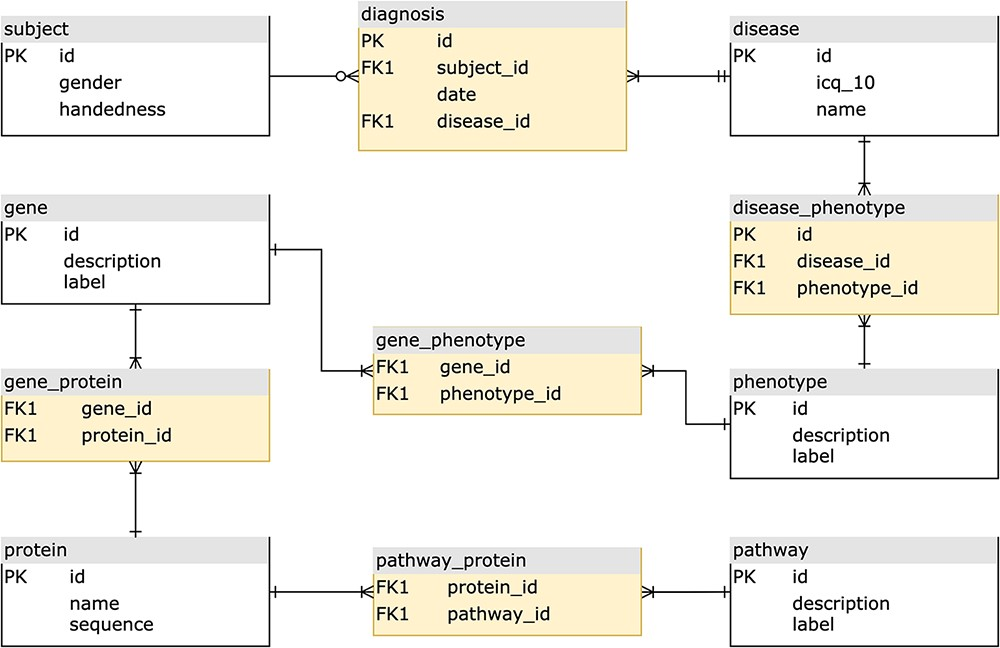
\includegraphics[width=0.5\linewidth]{images/DBRel.jpeg}}
    \hfill
    \subfloat[Base de données graphe]{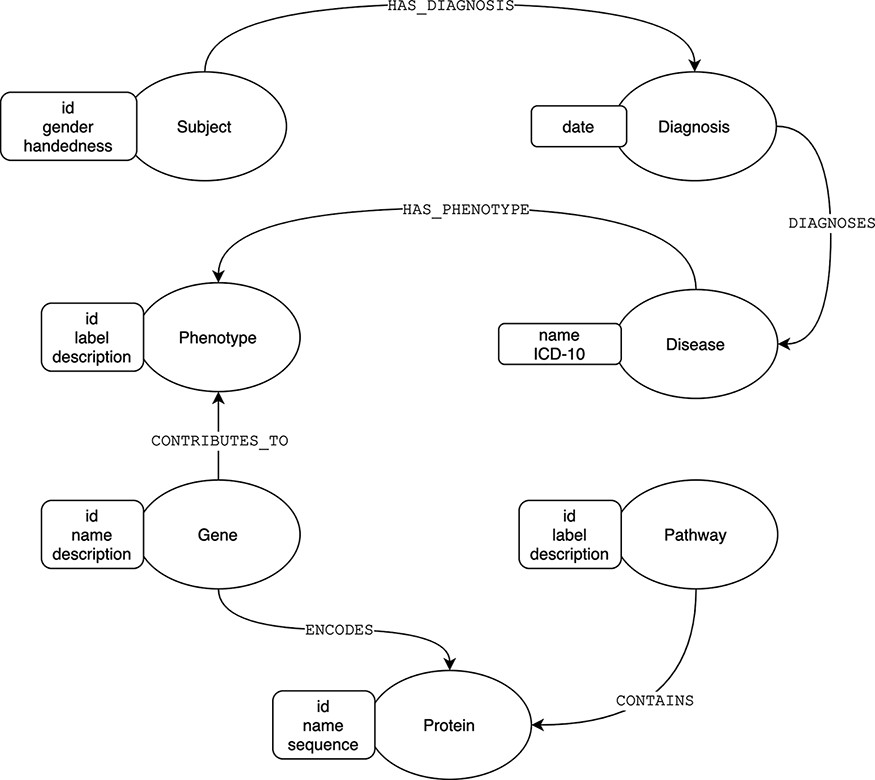
\includegraphics[width=0.4\linewidth]{images/DBGraph.jpeg}}
    \caption[Comparaison des modèles entre une base de données relationnelle et une base de données orientées graphe]{\textbf{Comparaison des modèles entre une base de données relationnelle et une base de données orientées graphe.} (a) Les tables contenant les informations sont représentées en blanc et les tables de jointure en jaune. (b) Les n\oe uds représentent les informations et les arêtes les relations (jointure). Extrait de \cite{timon-reina_overview_2021}}
    \label{fig:DBRel_vs_Graph}
\end{figure}

Parmi les bases de données et outils qui exploitent ces nouveaux modèles, GDM (Genomic Data Model) et GMQL (Genomic Metadata Query Language) illustrent bien l’évolution vers des architectures plus flexibles adaptées aux vastes ensembles de données génomiques \cite{masseroli_genometric_2015,masseroli_modeling_2016}. GDM est un modèle conçu pour gérer efficacement des données hétérogènes issues de la génomique, en intégrant à la fois des informations sur les séquences et leurs annotations. Dans cette perspective, GMQL se présente comme un langage de requête avancé permettant d’interroger ces bases de manière optimisée, facilitant l’exploration et l’intégration de données. Grâce à son interaction avec un modèle orienté graphe, GMQL améliore la capacité à interroger et à analyser de grands ensembles de données interconnectées, rendant possible l’identification rapide de corrélations complexes entre différentes sources d’information génomique.

\newpage

Dans le domaine du Web sémantique, BioRDF \cite{cheung_journey_2009} permet de modéliser et d'interconnecter des ressources issues des DB, biomédicales en particulier. Reposant sur le \textit{Ressource Description Framework} (RDF), cette approche permet de relier des concepts biologiques de manière standardisée, permettant ainsi une interopérabilité accrue entre les systèmes et l’extraction de nouvelles connaissances à partir de réseaux complexes. RDF est un modèle de données qui représente l'information sous forme de graphes. Chaque déclaration RDF est un triplet composé d'un sujet, d'un prédicat et d'un objet, ce qui forme naturellement une structure de graphe. BioRDF est utilisé dans diverses applications biologiques, y compris la création de \textit{workflows} bioinformatiques, l'annotation de séquences protéiques, et la modélisation de voies biologiques. Des outils comme Taverna \cite{oinn_taverna_2004} sont utilisés pour composer et exécuter ces workflows.

Un autre exemple de base de données orientée graphe est KEGG (\textit{Kyoto Encyclopedia of Genes and Genomes}), une ressource essentielle pour l’analyse des voies métaboliques, des interactions moléculaires et des relations entre gènes et maladies \cite{kanehisa_kegg_2025}. Contrairement aux bases relationnelles classiques, KEGG structure ses données sous forme de graphes de réseaux métaboliques, où les n\oe uds représentent des gènes, des protéines ou des petites molécules, interconnectés à travers des réactions biochimiques représentées par les arêtes. Cette organisation permet d’étudier le fonctionnement des systèmes biologiques à grande échelle et d’identifier des cibles potentielles pour le développement de nouvelles thérapies.

Ces bases de données sont également utilisées par des outils pour réaliser des analyses et des prédictions. C'est le cas de Spfy \cite{le_spfy_2018}, qui permet de prédire des phénotypes bactériens sur de nouveaux échantillons à partir d'une base de données MongoDB\footnote{MongoDB, une base orientée documents, adapté aux ensembles de données évolutifs et hétérogènes.} \cite{guo_mongodbs_2017}. Spfy est capable de prédire des caractéristiques phénotypiques importantes telles que le sérotype, le sous-type de la toxine Shiga (toxine sécrétée par les bactéries \textit{E. coli}), ainsi que la présence de facteurs de virulence et de déterminants de résistance aux antimicrobiens. Actuellement, la base de données contient plus de 10 000 génomes de \textit{Escherichia coli}.

Enfin, l’utilisation des bases de données orientées graphe s’est intensifiée avec des systèmes de gestion de base de données orientée graphe open-source comme Neo4J, qui a été largement exploité dans des projets tels que CovidGraph \cite{gutebier_covidgraph_2022}. Ce dernier est un réseau de connaissances conçu pour analyser la littérature scientifique, les bases de données biomédicales et les publications liées au SARS-CoV-2. En structurant ces informations sous forme de n\oe uds et d’arêtes, Neo4J permet d’explorer efficacement les relations complexes entre les études, les auteurs, les interactions moléculaires et les traitements potentiels contre la maladie.

Ces nouvelles approches et ces outils illustrent la transition vers des modèles de bases de données plus dynamiques et adaptés aux défis de la biologie moderne. Que ce soit par l’utilisation de langages de requête spécialisés, de technologies sémantiques, de modèles en graphe ou encore de bases NoSQL, ces solutions permettent une gestion plus efficace des données biomédicales et ouvrent la voie à des analyses plus approfondies dans le domaine des sciences de la vie.
